%\documentclass{article}
%\usepackage[T1]{fontenc}
%\usepackage[utf8]{inputenc}
%\usepackage{authblk}
%\usepackage{hyperref}
%\usepackage{booktabs}
%\usepackage{enumitem}
%\usepackage{geometry}
%\usepackage{graphicx}
%\usepackage[utf8]{inputenc}
%\usepackage[english]{babel}






\documentclass{subfiles}

\begin{document}
		

	\section{Introduction} \label{DASOS_Introduction}
	
	\par FW LiDAR systems have been available for a number of years but there still very few uses of FW LiDAR data. NERC-ARF has been acquiring airborne data for the UK and overseas since 2010 and it has more than 100 clients of new and archived data. Many clients request FW LiDAR data to be acquired, but despite the significant number of requests,the majority of research still only uses discrete LIDAR. Some of the factors regarding this slow takeup are:
	\begin{itemize}
		\item Typically FW datasets are 5 – 10 times larger than discrete data, with data sizes in the range of 50GB – 2.5TB GB for a single area of interest. NERC-ARF's datasets are up to 100GB each because most clients are research institutes but for commercial purposes each FW dataset is a couple of TB.
		\item Existing workflows are only able to work with the discrete data since the increased amount of information recorded within the FW LiDAR makes handling the quantity of data very challenging.
	\end{itemize}
	
	\par The open source software DASOS was developed to encourage foresters to use the FW LiDAR data. DASOS was named after the Greek word "$\delta\acute{a}\sigma o\varsigma$" (=forest) and it was firstly presented at the 36th International Symposium of Remote Sensing of the Enviroment, 2015. The main way of interpreting FW LiDAR data in DASOS is fundamentally different from the state-of-art available software packages. In a few words, the FW LiDAR data are voxelised by inserting the wave samples into a 3D discrete density volume. It accumulates intensity values from multiple shots and stores them into a 3D regular grid, resolving this way the problem with the sinusoidal footprints pattern of the Leica system. For more information please refer to the related paper at \url{<https://www.researchgate.net/publication/277347868_Alignment_of_hyperspectral_imagery_and_full-waveform_LIDAR_data_for_visualisation_and_classification_purposes>}
	
	\par This user guide aims to give an in depth understanding of DASOS's functionalities. In a few words there are three functionalities of DASOS: 
	\begin{enumerate}
		\item the construction of 3D polygon meshes; 
		\item the generation of 2D metrics aligned with hyperspectral images and
		\item the characterisation of objects using feature vectors. 
	\end{enumerate}
	
		\section{License} \label{License}
		
		\par DASOS is released under the GNU General Public Licence, Version 3. The full description of the usage licence is available here:\url{<https://github.com/Art-n-MathS/DASOS/blob/master/License.txt>}
		
		\par The following paper is the paper that introduced DASOS and it must be cited in any publications, software or other media using DASOS:
		
		Miltiadou M., Warren M. A., Grant M., Brown M., 2015, Alignment of Hyperspectral Imagery and full-waveform LiDAR data for visualisation and classification purposes, ISPRS Archives 36th International Symposium of	Remote Sensing of the enviroment. \cite{Miltiadou2015}
		
		\par Full paper available here: at:\url{<https://www.researchgate.net/publication/277347868_Alignment_of_hyperspectral_imagery_and_full-waveform_LIDAR_data_for_visualisation_and_classification_purposes>}
		
		
		
		\par The 1$^{st}$ sample dataset provided for testing was collected by the NERC Airborne Research and Survey Facility (ARSF). Copyright is held by the UK Natural Environment Research Council (NERC). The data are free for non-commercial use, but NERC-ARSF must be acknowledged in any publications, software or other media that make use of these data.
		
		\par The 2$^{nd}$ sample dataset provided by Interpine Group Ltd. Copyright is held by Interpine Group Ltd and the data are free for non-commercial use, but Interpine Group Ltd must be acknowledged for any publications, software or other media that make use of these data. 
		
		

	
	\section{Installation Guide} \label{Installation}
		\subsection {Windows}
		\par The windows executables are available at: \newline \url{<https://github.com/Art-n-MathS/DASOS/tree/master/DASOS_win>}
		 
		\par DASOS is a command line program and a terminal is required. For Windows XP, Vista and 7,  Command Prompt is the default terminal and it can be found from the search tab on the start menu. If you are using Windows 8, then right click on the start icon and choose 'Command Prompt'. Find the directory where DASOS is saved (the command 'dir' shows the files inside the current directory and the command 'cd' to open folder). Once you are in the correct directory, execute the following command to test that the program works fine. 
		
		\par \$: DASOS \texttt{-{}-}help  \footnote{the '\$:' is not included in the command. It just illustrate the start of a command in the terminal} 
		\par Information of all the available commands should be printed. If an error is occur, then either a .dll file is missing or DASOS is not supported at your computer.
		
		
		\subsection {Linux}
		\par The source code is available at: \url{<https://github.com/Art-n-MathS/DASOS>}.
		\par For compiling DASOS on Linux, there are three major dependencies: 
		\begin{enumerate}
		\item qmake-qt4 (or later release) / qtcreator 
		\item gmtl library - please update the .pro file to point to the correct directory
		\item -std=c++11
		\end{enumerate}
        \par Once those are installed compile DASOS as shown below: \newline
        \verb|$: qmake-qt4| \newline
        \verb|$: make| \newline		

        \par To test it, write the following command: 
        \par \$: DASOS \texttt{-{}-}help  
        \par Information of all the available commands should be printed. 
        

	\section{Instructions}\label{instructions}
	\subsection{Overview}\label{Overview}
	\par DASOS is a command line program and can either be used in Command Prompt on Windows or a Linux shell. 
	\par At first change directory (cd) to go to the directory DASOS is saved or compiled in. 
	Then for Windows run: 
	\par \verb|$: DASOS <arg1> <arg2> ... <argN>|
	\par or \verb|$: DASOS.exe <arg1> <arg2> ... <argN>|
	\par On Linux run:
	\par \verb|$: ./DASOS <ar1> <ar2> ... <argN>|
	\par For consistency this guide uses the 1$^{st}$ Windows example since all of the inputs, parameters and output arguments are the same for both Windows and Linux. 
	
	\par The tags of DASOS are divided into three groups: Inputs, Parameters and Outputs. 
		\begin{enumerate}
			\item Inputs (Section \ref{inputs})
			\item Parameters (Section \ref{parameters})
			\item Outputs (Section \ref{output})
		\end{enumerate} 
	\par Even though many tags are optional or contain default values, it's essential to follow the order <inputs> <parameters> <outputs> because if the outputs are defined first unexpected results may occur, due to adding outputs to the stack before parameters are initialised. The aforementioned Sections give an explanation of all the possible tags of DASOS. 
	
	\par Before proceeding to the explanation, it worth highlighting and numbering the three main outputs of DASOS. The corresponding sub-sections do not only explain the output but also the parameters that are only specific to the corresponding output. The user guide refers to those outputs using their numbers:
	
	\begin{enumerate}
			\item The generation of 3D polygonal meshes (Section \ref{PolygonalMesh})
			\item The 2D metrics aligned with Hyperspectral Imagery (Section \ref{DASOS_Alignment}
			\item The feature vectors for local inspection of data (Sub-section \ref{3Dpriors})		
	\end{enumerate}
	
		At the end of this guide, there is a list of limitations and the dependencies. 
	
	\subsection{Inputs}\label{inputs}
	\par The inputs are divided into FW LiDAR, Hyperspectral and fieldplots. The FW LiDAR are compulsory for all the functionalities of DASOS. The Hyperpsectral Inputs are optional for the 1st and 2nd output of DASOS (3D polygonal meshes and 2D metrics), while the fieldplots option is compulsory for the 3rd option, the feature vectors. 
	
	\par Table  \ref{table:DASOS_inputs} explains the tags for loading the FW LiDAR files files. Please note that it is compulsory to load one of those options. If more than one FW LiDAR files are loaded then it is essential to keep consistency between projects; load only one type of full-waveform LiDAR data simultaneously. Table \ref{table:DASOS_optional_inputs} outlines how the hyperspectral imagery is loaded, how to subtract a pre-calculated DTM and also how the file with fieldplots is loaded if the 3rd output option is chosen (feature vectors).
	
		
	\begin{table}[!htbp]
	{
		\centering
		\begin{tabular}{|p{3.4cm}|p{10.1cm}|}
			\toprule
			\textbf{Tags}  & \textbf{Description}  \\
			\midrule
			-las <file1> <file2> ... <fileN> & The name/directory of a number of LAS files (i.e. \verb|"C:\Dir Las\LAS1.las"|). It is further suggested to manually define the boundaries of the area of interest when multiples input files are loaded (use command -userLimits explained at Table \ref{table:parameters}). Otherwise the boundaries of the first LAS file loaded are used, which may lose data from subsequent input files. Furthermore DASOS only supports LAS1.3 with waveform packet format 4.    \\
				\cmidrule(r){1-1}\cmidrule(l){2-2}
			-pw <file1> <file2> ... <fileN> &  loads a number of pulsewave files (*.pls). Same rules apply as the -las tag  \\
				\cmidrule(r){1-1}\cmidrule(l){2-2}
			-volume <file> &   loads an exported volume, generated using DASOS, instead of reading a LAS or pulsewave file. \\
				\cmidrule(r){1-1}\cmidrule(l){2-2}
			-vols <dir> &   loads all the exported volume that are inside the given directory "dir". This option must and only be used for generating feature vectors (Section \ref{3Dpriors}). \\
		    \bottomrule
		\end{tabular}
		\caption{DASOS fundamental file inputs}
	   	\label{table:DASOS_inputs}
	}
	\end{table}
	
	
	\begin{table}
		\centering
		\begin{tabular}{|p{3.4cm}|p{10.1cm}|}
			\toprule
			\textbf{Tags}  & \textbf{Description}  \\
			\midrule
			-igm <igmFileName>  &  The name/directory of the .igm file that defines the geolocation of the hyperspectral pixels.  This file is an ENVI bil with latitude and longitude per pixel.\\
							\cmidrule(r){1-1}\cmidrule(l){2-2}
			-bil <bilFileName>  &  The name/directory of the .bil file that contains the hyperspectral cube.\\
							\cmidrule(r){1-1}\cmidrule(l){2-2}
			-fodis <fodisFile>   & The name/directory of the fodis (upward looking illumination sensor) .bil file for hyperspectral imagery \\
			\midrule
			\midrule
			-dtm <dtmFileName> & loads a pre-calculated DTM and subtracts it from the position of each waveform sample before importing it to the volume. Please note that the DTM file format must be .bil and saved into float pointing numbers. Potential further file format limitations may exist. This is optional. \\
			\midrule
			\midrule
			-csv <fieldplots.csv>  &  The input csv file that lists all the trees from a number of field-plot. This is a compulsory input for generating feature vectors;
				\\
			\bottomrule
		\end{tabular}
		\caption{Optional or output request dependant.}
		\label{table:DASOS_optional_inputs}
	\end{table}
		
			
			\newpage
		\subsection{General Parameters}\label{parameters}
			\par All the general parameters has been pre-defined and they are therefore optional. Nevertheless, parameters are advised to be adjusted for each project. Table \ref{table:parameters} contains information about all the parameters and how to modify the the voxelised FW LiDAR data during construction. Figures \ref{fig:SelectingRegionOfInterest} and \ref{fig:DASOS} show how the results are affected when these parameters are modified.
			
			
			\begin{table}[!htbp]
			\centering
				\begin{tabular}{|p{2.8cm}|p{10.7cm}|}
					\toprule
					\textbf{Tags}  & \textbf{Description}  \\
					\midrule
					-userLimits \newline<maxNorthY> \newline<minNorthY> \newline<maxEastX>\newline <minEastX> & User define boundaries of the area of interest. If not defined then the boundaries of the first file loaded are used (as defined in the header).\\
					\cmidrule(r){1-1}\cmidrule(l){2-2}
					-vl <voxelLength>   & The voxel length controls the resolution of the output; the bigger the voxel length is the lower the resolution and the number of cubes are. Default value is 2.5m\\
					\midrule
					-nl <noiseLevel>  &  The noise level is the threshold of the low level filtering applied during voxelisation. Default value is 25. Please note that the intensity of each wave sample is not transformed to volts. 
					Additionally, it is recommended to use the -exportPulses tag to export the amplitude of a few pulses and use those as sample data to define an appropriate noise threshold. \\
					\cmidrule(r){1-1}\cmidrule(l){2-2}
					-iso <isolevel>    & The iso-level is the intensity boundary that defines whether a voxel is empty or not. This is mostly used during polygonisation. The default value is zero. Please note that noise level and isosurface level are closely related but only the isolevel can be modified from an exported volume.\\			
					
					\bottomrule
				\end{tabular}
				\caption{Description of the all the available tags that customises voxelisation of the FW LiDAR data.}
				\label{table:parameters}
			\end{table}
			
			\begin{figure} [h!]
				\centering
				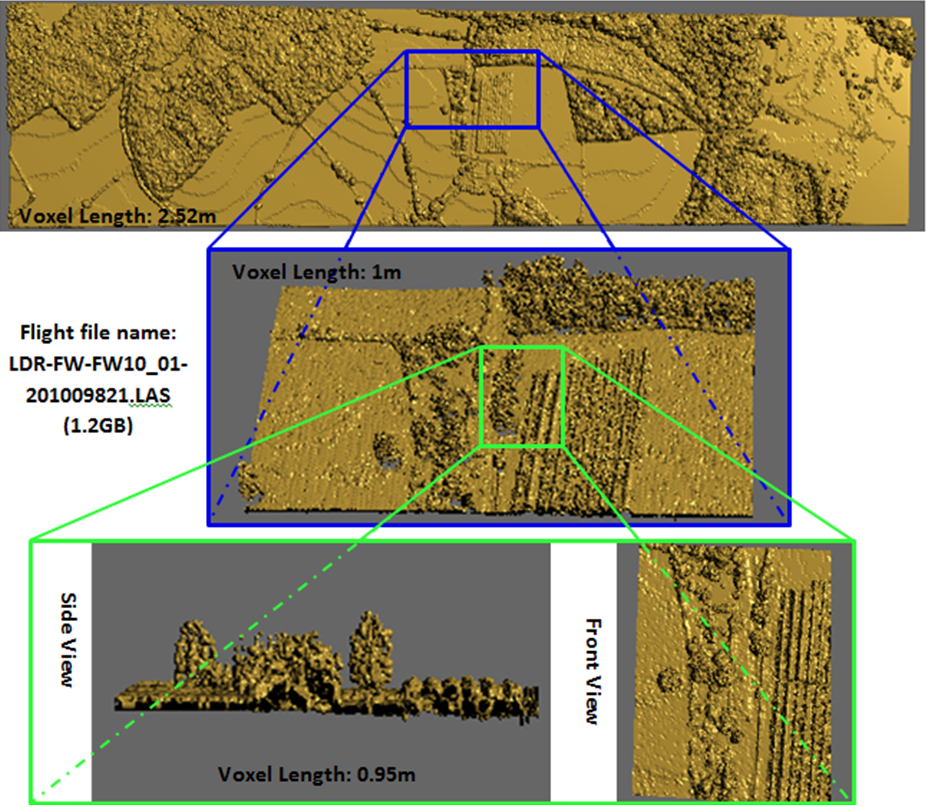
\includegraphics[width=.65\textwidth]{tex/Appendices/img/SelectingRegionOfInterest}
				\caption{Selecting Region of Interest}
				\label{fig:SelectingRegionOfInterest}
			\end{figure}			
			\begin{figure} [h!]
				\centering
				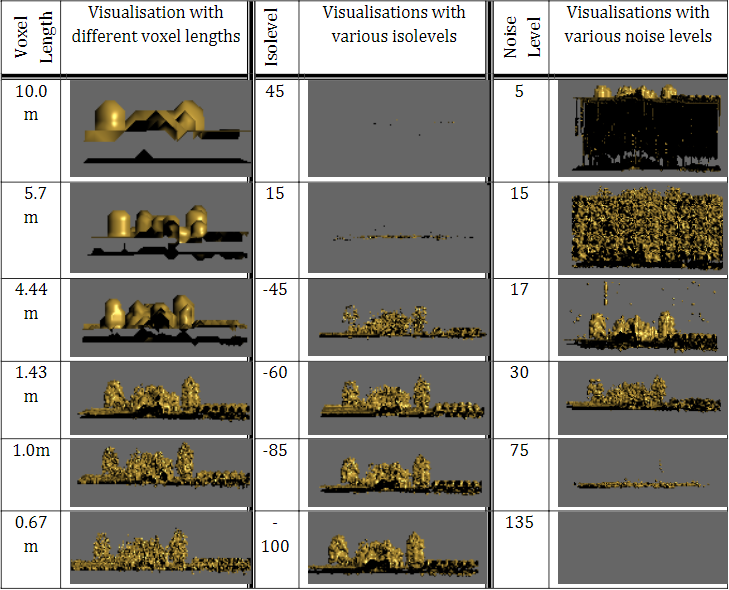
\includegraphics[width=.85\textwidth]{tex/Appendices/img/DASOS}
				\caption{Effect of modifying the user defined parameters; voxel length, isolevel and noise level.}
				\label{fig:DASOS}
			\end{figure}	
		
			
			\newpage
		
		\subsection{Outputs}\label{output}
		
		
			\par DASOS has three main outputs and three supplementary. At least one of them must be requested for the program to run. 
			
			\par The main outputs are the following:
			\begin{enumerate}
				\item \textbf{Polygonal Meshes}: exported into an .obj which is a standard graphics format that stores the vertices, edges and faces of the polygon. An image is also exported if hyperspectral data are loaded. (Section \ref{PolygonalMesh})
				\item \textbf{2D Metrics}: information about the scanned area in .asc format. If hyperspectral Images are loaded then aligned metrics from both datasets are available. (Section \ref{DASOS_Alignment})
				\item \textbf{List of Feature Vectors}: exported into .csv files. Each row of the spreadsheet contains information about a local 3D cylinderal or cubic area. (Section \ref{3Dpriors})
			\end{enumerate} 
		
		The three suplementary outputs are explained in Table \ref{table:supTags} while the main outputs are explained in Sections \ref{PolygonalMesh}, \ref{DASOS_Alignment} and \ref{3Dpriors} respectively.
		\begin{table}[!htbp]
			\centering
			\begin{tabular}{|p{2.9cm}|p{10.8cm}|}
				\toprule
				\textbf{Tags}  & \textbf{Description}  \\
				\midrule
				\texttt{-{}-}help & It prints a list with all the available commands along with their description.\\
				\midrule
				-exportPulses \newline<noOfPulses> \newline<fileName.csv> & Method that exports a number of pulses into a .csv file. The input <noOfPulses> the number of sample pulses to be exported into the <fileName.csv> file. It is used for deciding the noise level threshold for each project. \\
				\cmidrule(r){1-1}\cmidrule(l){2-2}
				-exportVolume c\newline <volumeFileName> & Exports the volume into an ASCII file to speed up future interpolation of the data. 'c' refers to compressed and it's an implicit functionality. If 'c' is not included then a non compressed file is exported, which sometimes is too big to be read back into DASOS. Therefore 'c' should always be included. \\	
				\bottomrule		
			\end{tabular}
			\caption{The supplementary ouput options of DASOS.}
			\label{table:supTags}
		\end{table}
	
		
		\newpage
		
		\subsubsection{Polygonal Meshes}\label{PolygonalMesh}
        
        
        
		\begin{longtable}
			{|p{2.5cm}|p{5.2cm}|p{5.8cm}|}
				\toprule
       			\multicolumn{3}{|c|}{\textbf{1st Main Output: 3D Polygon Mesh Generation }} \\
       			\midrule
				\textbf{Tags}&\textbf{Description} & \textbf{Output Example}\\ 
				\midrule
					-obj \newline<objFileName> & The input <objFileName> is the name of the .obj file where the polygon representation of the LiDAR file will be exported to. A texture is also exported when hyperspectral images are loaded. & \raisebox{-\totalheight}{\adjincludegraphics[width=\linewidth]{img/NewForest}} \\
				
			\bottomrule
		\caption{Description of generating polygonal meshes and example outputs}
		\label{table:PolMeshes}
	\end{longtable}
	
	
	\newpage
	
	 	\subsubsection{2D Metrics Aligned with Hyperspectral Imagery}\label{DASOS_Alignment}
	 	
	 	
	 	
			\begin{longtable}	 	
		 	{|p{3.2cm}|p{10.4cm}|}
	 			\toprule
	 			\multicolumn{2}{|c|}{\textbf{2nd Main Output: Generation of 2D metrics}} \\
	 			\multicolumn{2}{|c|}{\textbf{aligned with hyperspectral imagery }} \\
	 			\midrule
	 			\textbf{Tags}  & \textbf{Description}  \\
	 			
	 			\midrule
	 			-map <type>\newline <outputName>    & The available types are the following. Full description of each option is given in Table \ref{table:AlignedMetrics} along with output examples. 
	 			\begin{itemize}[noitemsep]
	 				\item \verb|HEIGHT|
	 				\item \verb|THICKNESS|
	 				\item \verb|DENSITY |
	 				\item \verb|FIRST_PATCH|
	 				\item \verb|LAST_PATCH|
	 				\item \verb|AVERAGE_HEIGHT_DIFFERENCE|
	 				\item \verb|LOWEST_RETURN|
	 				\item \verb|INTENSITY_MAX|
	 				\item \verb|INTESNSITY_AVG|
	 				\item \verb|HYPERSPECTRAL_MEAN|
	 				\item \verb|NDVI|
	 				\item \verb|ALL_FW| 
	 			\end{itemize} \\
	 			&  All the maps are exported into .asc format and can be loaded into QGIS and other software packages. The \verb|ALL_FW| option generates one metric for each available full-waveform LiDAR related metric and their names are: outputName+metricsType+.asc \newline
	 			Table \ref{table:AlignedMetrics} explains what each metric is and gives output examples.\\
	 			\cmidrule(r){1-1}\cmidrule(l){2-2}
	 			-map \newline HYPERSPECTRAL \newline <band>\newline <outputName> & The hyperspectral map needs an extra parameter defining which band will be output. \\
	 			
	 			
	 			\bottomrule
	 		\caption{DASOS ouput options}
	 		\label{table:outputs}
	 	\end{longtable}
	 	
	 
	 	\newpage
	 		\begin{longtable}
	 				{| p{7.9cm}  | p{5.6cm} | }
	 			\toprule
	 		\textbf{Metric Description}&\textbf{Example} \\ 
	 		
			\midrule
	 		\textbf{HEIGHT (DEM): } \newline The distance between the top non-empty voxel and the lower boundaries of the volume. & \raisebox{-\totalheight}{\adjincludegraphics[width=\linewidth,trim={{.1\width} 0 {.25\width} 0},clip]{img/metrics/HEIGHT}}  \\ 
	 		
	 		\cmidrule(r){1-1}\cmidrule(l){2-2}
	 		\textbf{THICKNESS: } \newline The distance between  the  first  and  last  non  empty  voxels  in every   column of the   3D   volume.& \raisebox{-\totalheight}{\adjincludegraphics[width=\linewidth,trim={{.1\width} 0 {.25\width} 0},clip]{img/metrics/THICKNESS}} \\ 
	 			 		
	 		\cmidrule(r){1-1}\cmidrule(l){2-2}
	 		\textbf{DENSITY:} \newline Number of non-empty voxel over all voxels within  the  range  from the first to last non-empty voxels. &       \raisebox{-\totalheight}{\adjincludegraphics[width=\linewidth,trim={{.1\width} 0 {.25\width} 0},clip]{img/metrics/DENSITY}} \\ 
	 		
	 		\cmidrule(r){1-1}\cmidrule(l){2-2}
	 		\textbf{FIRST\_PATCH: } \newline The number of non-empty adjacent voxels, starting from the first/top non-empty voxel in that column. &         					\raisebox{-\totalheight}{\adjincludegraphics[width=\linewidth,trim={{.1\width} 0 {.25\width} 0},clip]{img/metrics/FIRST_PATCH}} \\ 
	 		 		
	 		\cmidrule(r){1-1}\cmidrule(l){2-2}
	 		 \textbf{LAST\_PATCH: } \newline The number of non-empty adjacent voxels, starting from   the last/lower   non-empty   voxel in   that column.& \raisebox{-\totalheight}{\adjincludegraphics[width=\linewidth,trim={{.1\width} 0 {.25\width} 0},clip]{img/metrics/LAST_PATCH}}  \\
	 		
	 		\cmidrule(r){1-1}\cmidrule(l){2-2}
	 		  \textbf{AVERAGE\_HEIGHT\_DIFFERENCE:}\newline An edge detection algorithm. &         	\raisebox{-\totalheight}{\adjincludegraphics[width=\linewidth,trim={{.1\width} 0 {.25\width} 0},clip]{img/metrics/AverageHeightDiff}} \\ 
	 		
	 		\cmidrule(r){1-1}\cmidrule(l){2-2}
	 		 \textbf{LOWEST\_RETURN } \newline The height of the lowest non empty voxel (the actual heights are very low and close to each but the example image has been scaled and the different seems bigger)&  \raisebox{-\totalheight}{\adjincludegraphics[width=\linewidth,trim={{.1\width} 0 {.25\width} 0},clip]{img/metrics/LOWEST_RETURN}}  \\
	 		
	 		\cmidrule(r){1-1}\cmidrule(l){2-2}
	 		\textbf{INTENSITY\_MAX } \newline The maximum intensity of each column& \raisebox{-\totalheight}{\adjincludegraphics[width=\linewidth,trim={{.1\width} 0 {.25\width} 0},clip]{img/metrics/metric_INTENSITY_MAX}} \\
	 		
	 		\cmidrule(r){1-1}\cmidrule(l){2-2}
	 		\textbf{INTENSITY\_AVG } \newline The average intensity per column& \raisebox{-\totalheight}{\adjincludegraphics[width=\linewidth,trim={{.1\width} 0 {.25\width} 0},clip]{img/metrics/metric_INTENSITY_AVG}} \\
	 		
	 		
	 		\cmidrule(r){1-1}\cmidrule(l){2-2}
	 		 \textbf{HYPERSPECTRAL\_MEAN} \newline The mean of the hyperspectral spectrum.& \raisebox{-\totalheight}{\adjincludegraphics[width=\linewidth,trim={{.1\width} 0 {.25\width} 0},clip]{img/metrics/HYPERSPECTRAL_MEAN}} \\ 
	 		
	 		\cmidrule(r){1-1}\cmidrule(l){2-2}
	 		\textbf{NDVI } \newline  The Normalised Difference Vegetation Index indicates whether green vegetation exists or not and it is derived from the electromagnetic spectrum as follow:
	 			\begin{eqnarray}
	 			NDVI = \dfrac{NIR-VIS}{NIR+VIS}
	 			\end{eqnarray}
	 			where the NIR is the near-infrared region of the spectrum (700-2500nm) and VIS is the Visible/Visual spectrum (430-770) 
	 			\cite{Crippen1990_NDVI}.& \raisebox{-\totalheight}{\adjincludegraphics[width=\linewidth,trim={{.1\width} 0 {.25\width} 0},clip]{img/metrics/NDVI}}  \\ 
	 		
	 	
	 		
	 		
	 		\cmidrule(r){1-1}\cmidrule(l){2-2}
		 	\textbf{HYPERSPECTRAL} \newline A single user defined hyperspectral band. & \raisebox{-\totalheight}{\adjincludegraphics[width=\linewidth,trim={{.1\width} 0 {.25\width} 0},clip]{img/metrics/hy235}} \\ 
	 			
	 			\bottomrule
	 			
	 			\caption{Description of generating polygonal meshes and example outputs}
	 			\label{table:AlignedMetrics}
	 		\end{longtable}
	 		
	 	\newpage
		\subsubsection{List of Feature Vectors}\label{3Dpriors}
		\par This is useful for characterising object inside the 3D space (e.g. trees). For each column of the voxelised FW LiDAR, information around its local area are exported. 
		
		
		\par Similar to the previous functionalities of DASOS, the program requires <inputs> <parameters> and <outputs>. Those requirements are described in Tables \ref{tbl:PriorsInputs}, \ref{tbl:PriorsParameters} and \ref{tbl:PriorsOutputs} respectively. Please note that these inputs are also described with the rest of the inputs in Section \ref{inputs}.
		
		
		\begin{longtable}
		 	{|p{3.1cm}|p{10.5cm}|}
						
			\toprule
			\multicolumn{2}{|c|}{\textbf{3rd Main Output: List of Feature Vectors - Inputs }} \\
			\midrule
		
			\textbf{Tags} & \textbf{Description} \\ 
			\cmidrule(r){1-1}\cmidrule(l){2-2}
			 -vols <volDir>  &  the directory of the volume of interest generated beforehand. 
			 \\
			\cmidrule(r){1-1}\cmidrule(l){2-2}
			 -icsv \newline <fieldplots.csv> & the input csv file that contains all information about the fieldplots. 
			    \\
			\bottomrule
			\caption[DASOS's functionalities]{Explanation of how to define the two compulsory inputs to get the 3rd main output of DASOS}
			\label{tbl:PriorsInputs}	
		\end{longtable}
		
		\par Figure \ref{fig:fieldplot} shows an example of a file with fielplots. A file may contain multiple fieldplots, but it has to have at least 6 columns: the 3 columns define the fieldplot (northing, easting and radius) and the rest give information about the trees (northing, easting and class). The order of the columns has no significance. Figure \ref{fig:fieldplot} shows an example. The labels of the those columns could vary and can be defined as explained in Table \ref{tbl:PriorsParameters}. 
		
		  \begin{figure} [h!]
		  	\centering
		  	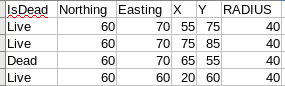
\includegraphics[width=0.45\textwidth]{tex/Appendices/img/fieldplot}
		  	\caption{Example of fieldplot input}
		  	\label{fig:fieldplot}
		  \end{figure}	
		
		\par {\color{blue} Additionally, the size and shape of the investigated area from where the features are extracted is user defined and Table \ref{tbl:PriorsParameters} lists all the related, modifiable parameters.}
		
					\newpage
			\begin{longtable}
				{|p{3.1cm}|p{11cm}|}
				
				\toprule
				\multicolumn{2}{|c|}{\textbf{3rd Main Output: List of Feature Vectors - Parameters }} \\
				\midrule
				
				\textbf{Tags} & \textbf{Description} \\ 
				\cmidrule(r){1-1}\cmidrule(l){2-2}
				-column <label> & the label of the column that defines the class of each entry (e.g. <label> = isDead) \\
				\cmidrule(r){1-1}\cmidrule(l){2-2}
				-class <className or ALL> & the name of the class (e.g. dead or alive) of interest or ALL. If a class is chosen, then only the columns that contain a tree of that class are taken into consideration; a feature list is exported for each tree that belongs to this class only. The ALL option is the area of interest and generates a template for each column that lies inside the voxelised space. \\
				
				\cmidrule(r){1-1}\cmidrule(l){2-2}
				-ttype  square <x> <y> <z> & generates a feature vector derived from a cuboid area of size x, y, z voxels. The systems finds the first non empty voxel starting from the top of the column. By default it moves one voxel upwards and sets that to be the top of the cuboid/cylinder. It is highly recommended to use odd numbers, otherwise the centre of the cuboid/cylinder will be wrongly set and unpredicted output values may occur. 		\\		
				\cmidrule(r){1-1}\cmidrule(l){2-2}
				-ttype cylinder <h> <r> & generates a cylindrical template with height h and diameter $(2 \times r + 1)$ voxels and height $h$. The systems finds the first non empty voxel starting from the top of the column. By default it moves one voxel upwards and sets that to be the top of the cuboid/cylinder. \\
				\cmidrule(r){1-1}\cmidrule(l){2-2}
				-mheight <n> & moves the template into the y-axis $n$ voxels upwards instead of one which is the default. The value $n$ must be a positive number.\\
				\cmidrule(r){1-1}\cmidrule(l){2-2}
				-eparameters <raw or processed> & the ‘raw’ option saves all the intensity values of the template and the ‘processed’ option saves parameters derived from the raw intensities. Table \ref{tbl:PriorsOutExplanation} explains how each processed parameters is derived. \\
				\bottomrule
				\caption[DASOS's functionalities]{Explanation on how to Modify the Parameters of the 3rd Main Output of DASOS}
				\label{tbl:PriorsParameters}	
			\end{longtable}
			
			\newpage
				\begin{longtable}
					{|p{3.1cm}|p{11cm}|}
					\toprule
					\multicolumn{2}{|c|}{\textbf{3rd Main Output: List of Feature Vectors  - Outputs }} \\
					\midrule
					\textbf{Tags} & \textbf{Description} \\ 
					\cmidrule(r){1-1}\cmidrule(l){2-2}
					-ocsv <nameStart> & For each .vol file found in the given directory (using -vols), a csv file is exported. The name of each file exported is:\newline <nameStart> + <volFileName> + ”.csv” \newline and it contains the list of the feature vectors generated from the corresponding volume \\
					\bottomrule
					\caption{Explanation of the tag that exports the list of feature vectors}
					\label{tbl:PriorsOutputs}	
				\end{longtable}
	     Figure \ref{fig:PriorExample} shows examples of two exported list of feature vectors: one with processed parameters and one with raw intensities. In each .csv file exported, each line is a feature vector. The first column is its ID as it defined during run time. The second and third columns define the centroids of each investigated local area (cuboid/cylinder). The other columns contain either processed or raw parameters. If they are processed, then information like mean height and standard deviation of heights are listed. Table \ref{tbl:PriorsOutExplanation} is a full list of all the proccessed parameters. If the parameters are raw, then the corresponding voxel intensity values are exported. The label of each voxel is "v\_x\_y\_z", where "v\_0\_0\_0" is the lower voxel of the cuboid/cylinder and it has the minimum easting and northing it as well. 
	     	
	
	     \begin{figure} [h!]
	     	\centering
	     	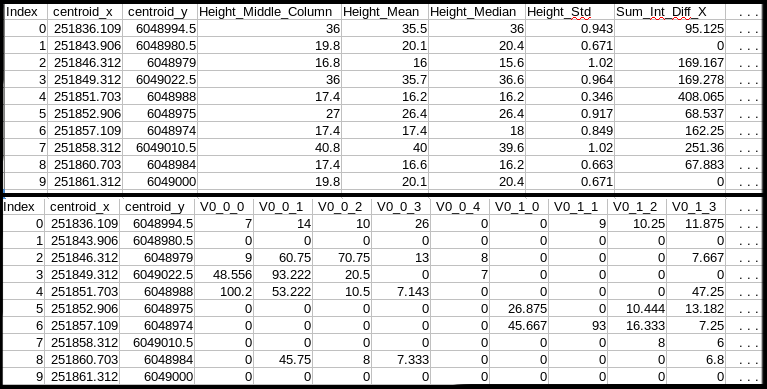
\includegraphics[width=0.93\textwidth]{tex/Appendices/img/PriorsBoth}
	     	\caption{Example of .csv files with a list of feature vectors exported. }
	     	\label{fig:PriorExample}
	     \end{figure}		
	
	
		
		\newpage
		\begin{longtable}
			{|p{4.65cm}|p{8.85cm}|}
			\toprule
			\multicolumn{2}{|c|}{\textbf{Explanation of the List of Feature Vectors Output }} \\
				\multicolumn{2}{|c|}{\textbf{ with the Processed Intensities}} \\
			\midrule
			\textbf{Label} & \textbf{Description} \\ 
			\cmidrule(r){1-1}\cmidrule(l){2-2}
			Height\_Middle\_Column& The height of the middle column of the cuboid/cylinder
			\\
			\cmidrule(r){1-1}\cmidrule(l){2-2}
			Height\_Mean& The Mean height of all the columns included in the template\\
			\cmidrule(r){1-1}\cmidrule(l){2-2}
			Height\_Median& The Median height of all the columns included in the template
			\\
			\cmidrule(r){1-1}\cmidrule(l){2-2}
			Height\_Std&The Standard Deviation of the heights of the columns included in the template \\
			\cmidrule(r){1-1}\cmidrule(l){2-2}
			Sum\_Int\_Diff\_X& The Mirror Summed Difference of the intensities using the middle column in the x-axis as the axis of symmetry \\
			\cmidrule(r){1-1}\cmidrule(l){2-2}
			Sum\_Int\_Diff\_Y& The Mirror Summed Difference of the intensities using the middle column in the y-axis as the axis of symmetry\\
			\cmidrule(r){1-1}\cmidrule(l){2-2}
			Sum\_Int\_Diff\_Z& The Mirror Summed Difference of the intensities using the middle column in the z-axis as the axis of symmetry\\
			\cmidrule(r){1-1}\cmidrule(l){2-2}
			Max\_Int& The maximum intensity found inside the cuboid/cylinder\\
			\cmidrule(r){1-1}\cmidrule(l){2-2}
			Min\_Int& The minimum intensity found inside the cuboid/cylinder\\
			\cmidrule(r){1-1}\cmidrule(l){2-2}
			Ave\_Int& The average intensity of the voxels that contain an intensity above the isolevel\\
			\cmidrule(r){1-1}\cmidrule(l){2-2}
			Median\_Int& The median intensity of the voxels\\
			\cmidrule(r){1-1}\cmidrule(l){2-2}
			Per\_Int\_Above\_Iso& Percentage of voxels that contain an intensity above the isolevel\\
			\cmidrule(r){1-1}\cmidrule(l){2-2}
			Dis\_Mean& Mean distance from the central voxel to every voxel that contain san intensity above the isolevel  \\
			\cmidrule(r){1-1}\cmidrule(l){2-2}
			Dis\_Median& Median distance from the central voxel to every voxel that contains an intensity above the isolevel \\
			\cmidrule(r){1-1}\cmidrule(l){2-2}
			Dis\_Std& The Standard Deviation of the distances between the central voxel and every voxel that contains an intensity above the isolevel\\
			\cmidrule(r){1-1}\cmidrule(l){2-2}
			Top\_Patch\_Len\_Middle\_Col& The length of the top patch of the middle column of the cuboid/cylinder\\
			\cmidrule(r){1-1}\cmidrule(l){2-2}
			Top\_Patch\_Len\_Mean& The Mean length of all the top patches\\
			\cmidrule(r){1-1}\cmidrule(l){2-2}
			Top\_Patch\_Len\_Median& The Median length of all the top patches \\
			\cmidrule(r){1-1}\cmidrule(l){2-2}
			Top\_Patch\_Len\_Std& The Standard Deviation of all the top patches \\
			\cmidrule(r){1-1}\cmidrule(l){2-2}
			Mirror\_Diff\_X\_Mean& The Mean Mirror Difference of the voxel intensities with the middle column of the x-axis as the symmetric axis\\
			\cmidrule(r){1-1}\cmidrule(l){2-2}
			Mirror\_Diff\_X\_Median& The Median Mirror Difference of the voxel intensities with the middle column of the x-axis as the symmetric axis \\
			\cmidrule(r){1-1}\cmidrule(l){2-2}
			Mirror\_Diff\_X\_Std& The Standard Deviation Mirror Difference of the voxel intensities with the middle column of the x-axis as the symmetric axis \\
			\cmidrule(r){1-1}\cmidrule(l){2-2}
			Mirror\_Diff\_Y\_Mean&  The Mean Mirror Difference of the voxel intensities with the middle column of the y-axis as the symmetric axis \\
			\cmidrule(r){1-1}\cmidrule(l){2-2}
			Mirror\_Diff\_Y\_Median&The Median Mirror Difference of the voxel intensities with the middle column of the y-axis as the symmetric axis 
			 \\
			\cmidrule(r){1-1}\cmidrule(l){2-2}
			Mirror\_Diff\_Y\_Std& The Standard Deviation Mirror Difference of the voxel intensities with the middle column of the y-axis as the symmetric axis\\
			\cmidrule(r){1-1}\cmidrule(l){2-2}
			Mirror\_Diff\_Z\_Mean&The Mean Mirror Difference of the voxel intensities with the middle column of the z-axis as the symmetric axis \\
			\cmidrule(r){1-1}\cmidrule(l){2-2}
			Mirror\_Diff\_Z\_Median& The Median Mirror Difference of the voxel intensities with the middle column of the z-axis as the symmetric axis \\
			\cmidrule(r){1-1}\cmidrule(l){2-2}
			Mirror\_Diff\_Z\_Std& The Standard Deviation of the Mirror Difference of the voxel intensities with the middle column of the z-axis as the symmetric axis \\
			\bottomrule
			\caption{Explanation of the processed parameter exported within a feature vector}
			\label{tbl:PriorsOutExplanation}	
		\end{longtable}
		
		
	\section{Exercises}\label{exercises}
	
	   	\subsection{Sample Data}
	   	These exercises will give you an in depth understanding of DASOS, while working with real examples. At first, copy the folder \verb|"DASOS_userGuide"| into your \verb|C:\| drive. This folder is available to download from \url{<https://github.com/Art-n-MathS/DASOS/tree/master/DASOS_win>}: To ease typing, all the example commands are given in the ExerciseCommands.bat file, which can be opened in a text editor.
	   	
	   	There are three datasets provided for the following exercises and they are available at: \url{<https://www.dropbox.com/sh/hzpl16gue5xvjmb/AADQsJOsqKkx0lCX4mJjvBPVa?dl=0>} and \url{<  		https://plymouthmarinelaboratory.webex.com/plymouthmarinelaboratory/j.php?MTID=m305f59dda16e653b2946c6a3b00e93f4>}. Please copy the data inside the directory <DASOS/DASOS\_win/SampleDATA> check that the following files are included:
	   	
	   	\begin{enumerate}
	   		\item 1$^{st}$ sample dataset inside < \verb|C:\DASOS_userGuide\SampleDATA\DATASET_1|>: 
	   		\begin{enumerate}
	   			\item \verb|LDR-FW-FW10_01-201009821.LAS|
	   			\item \verb|e098211b_FODIS.bil|
	   			\item \verb|e098211b_FODIS.bil.hdr|
	   			\item \verb|e098211b_masked.bil|
	   			\item \verb|e098211b_masked.bil.hdr|
	   			\item \verb|e098211b_osgn.igm|
	   			\item \verb|e098211b_osgn.igm.hdr|
	   			\item \verb|Readme.txt|
	   		\end{enumerate}
	   		\item 2$^{nd}$ sample dataset inside < \verb|C:\DASOS_userGuide\SampleDATA\DATASET_2|>
	   		\begin{enumerate}
	   			\item \verb|Australia_1.pls|
	   			\item \verb|Australia_1.wvs|
	   			\item \verb|Australia_1_dtm.bil|
	   			\item \verb|Australia_1_dtm.hdr|
	   			\item \verb|Australia_2.las|
	   			\item \verb|Australia_2.wdp|
	   			\item \verb|Australia_2_dtm.bil|
	   			\item \verb|Australia_2_dtm.hdr|
	   			\item \verb|Australia_3.las|
	   			\item \verb|Australia_3.wdp|
	   		\end{enumerate}
	   		
	   		\item 3$^{rd}$ sample dataset inside < \verb|C:\DASOS\_userGuide\SampleDATA\DATASET_3|>
	   		\begin{enumerate}
	   			\item \verb|myTestVol_.vol|
	   			\item \verb|myTestVol_flat.vol|
	   			\item \verb|testFieldplot.csv|
	   		\end{enumerate}
	   		
	   	\end{enumerate}
	   	
	   	
	    \par Information about data usage and related license are given in Section \ref{License}
	   	
		\par Once all the files are copied across, open the command Prompt and type:\newline
		\verb|$: cd C:\DASOS_userGuide\DASOS| \newline 
		This will bring you to our working directory. In case you are using a different directory then go to your work directory inside the folder DASOS and the rest of the commands should work OK. 
        \newline\newline
		A full guide of all the available tags is given with the following command. \newline
		\verb|$: DASOS --help| \newline
		 The same information can be found inside the Readme.txt file and this User Guide (Section \ref{instructions} ).
		
	   	\subsection{Exercises}
		\subsubsection{Deciding Noise Threshold}
		The following examples export the amplitudes of 12 pulses into a .csv file to help us decide what noise threshold to use. \newline\newline
		\verb|$:DASOS -las ..\SampleDATA\DATASET_1\LDR-FW-FW10_01-201009821.LAS |\newline \verb| -exportPulses 12   ..\LAS21pulsesSamples.csv|
		\newline\newline
		\verb|$: DASOS -las ..\SampleDATA\DATASET_2\Australia_2.las -exportPulses 12|\newline \verb|   ..\Australia_2_pulsesSamples.csv|
				
		\subsubsection{Exporting metrics from DASOS}
		The following commands export a height map into .asc files. These files can be used in QGIS. This will give us the location of the flightlines and the relation between them.
		\newline\newline
		\verb|$: DASOS -las ..\SampleDATA\DATASET_2\Australia_2.las -nl 6 -vl 2 -map |\newline \verb| height   ..\Australia_2_vl2_height|				
		\newline\newline
		\verb|$: DASOS -las ..\SampleDATA\DATASET_2\Australia_3.las -nl 6 -vl 2 -map|\newline \verb| height   ..\Australia_3_vl2_height|
		\newline\newline
		Generating a single map at the beginning is useful for deciding which flightlines lie inside the area of interest. 
		
		\subsubsection{Loading Multiple Flightlines}
		As mentioned before, for loading multiple flightlines it is suggested to manually define the boundaries of the area of interest. The following command loads two flightlines, generates a volume from the area of interest and exports it into the Australia2-3.vol file.
		\newline\newline
		\verb|$: DASOS -las ..\SampleDATA\DATASET_2\Australia_3.las|\newline \verb|   ..\SampleDATA\DATASET_2\Australia_2.las -nl 6 -vl 2 -iso 4 -userLimits |\newline \verb| 6199990  6199639  762405 761951 -exportVolume c ..\Australia2-3.vol|
		
		\subsubsection{Exporting Metrics}
		The following command loads the pre-computed volume and creates a height map and all the FW related metrics. Please note that height is also a FW related metric, therefore it will be created twice. \newline
		\verb|$: DASOS -volume ..\Australia2-3.vol -map height ..\Australia2-3 -map |\newline \verb|all_fw   ..\Australia2-3|
		
		\subsubsection{Subtracting Pre-computed Digital Terrain Model}
		The next command loads two LAS files, a pre-computed DTM file is subtracted from the wave samples' positions while the volume is created, the volume is exported into the \verb|Australia2-3_dtm.vol| file and finally it exports a height metric.\newline
		Please note that when a DTM is introduced, a new volume must be created. Since the volumetric files are raster data and contain no information about pulses.
		\newline\newline 		
		\verb|$: DASOS -las ..\SampleDATA\DATASET_2\Australia_3.las|\newline \verb|  ..\SampleDATA\DATASET_2\Australia_2.las   -dtm |\newline \verb| ..\SampleDATA\DATASET_2\Australia_2_dtm.bil -nl 6 -vl 2 -iso 4|\newline \verb| -userLimits   6199990  6199639 762405 761951 -exportVolume |\newline \verb|c ..\Australia2-3_dtm.vol -map  height   ..\Australia2-3_vl2_dtm_height|
		\newline\newline
		You may then use the same volume to export more metrics:\newline
		\verb|$: DASOS -volume ..\Australia2-3_dtm.vol -map AVERAGE_HEIGHT_DIFFERENCE |\newline \verb|   ..\Australia2-3_dtm_AVG_height_diff|
		
		\subsubsection{Pulsewave Data}
		As mentioned before, it is suggested to first export the amplitudes of a few pulses to decide on an appropriate noise threshold.\newline
		\verb|$: DASOS -pw ..\SampleDATA\DATASET_2\Australia_1.pls -exportPulses 15 |\newline \verb|   ..\PLS_amplitudeSamples.csv|
		\newline\newline
		And then you can generate the desired metrics:\newline
		\verb|$: DASOS -pw ..\SampleDATA\DATASET_2\Australia_1.pls -nl 5 -dtm |\newline \verb|   ..\SampleDATA\DATASET_2\Australia_1_DTM_1m.bil -vl 3 -map thickness |\newline \verb| PLS_vl3_thickness   -exportVolume ..\Australia_1_vl3_dtm.vol|\newline
		
		\subsubsection{Polygon Representation}
		DASOS create 3D polygon representation using the '-obj' tag. The 3D polygon representations are exported into .obj format, which can be visualised using animation software packages. For this workshop we are using Meshlab because it is a free tool and it can handle millions of triangles.\newline
		Meshlab is available to download from here: \url{<http://meshlab.sourceforge.net/>} and it is also included into our working directory \verb|"DASOS_userGuide"|.\newline
		An example of generating polygons is given below:\newline
		\verb|$: DASOS -las ..\SampleDATA\DATASET_1\LDR-FW-FW10_01-201009821.LAS -nl 20|\newline \verb| -vl 1.7  -obj   ..\LAS21.obj -exportVolume c ..\LAS21_vl1.7.vol|\newline
		The generated volume is also saved because we need it for the following exercises. 
		
		
	    \subsubsection{Hyperspectral Imagery}
	    \par One of the key functionalities of DASOS is the alignment with the hyperspectral imagery. DASOS can export 3D coloured polygon representations and aligned metrics between FW LiDAR and hyperspectral data. 
	    
	   \par For the 3D coloured polygon representations you must not use any directory for the exported .obj file Analysisname because the link between the texture and the .obj file will not work. Here is an example:\newline
	    \verb|$: DASOS -volume ..\LAS21_vl1.7.vol -bil |\newline \verb| ..\SampleDATA\DATASET_1\e098211b_masked.bil -igm |\newline \verb|   ..\SampleDATA\DATASET_1\e098211b_osgn.igm -fodis |\newline \verb|   ..\SampleDATA\DATASET_1\e098211b_FODIS.bil -rgb 240 78 23 -obj |\newline \verb|   LAS21_coloured.obj|\par 
	    \par The LAS21.obj file will be saved into the current directory, which in our case is: \newline \verb|C:\DASOS_userGuide\DASOS|. 
	    \par Please note that the following command should give the same results, but as mentioned before importing an exported volume is faster than generating from scratch. \newline
	    \verb|$: DASOS -las ..\SampleDATA\DATASET_1\LDR-FW-FW10_01-201009821.LAS -nl 20 |\newline \verb|-vl 1.7  -bil    ..\SampleDATA\DATASET_1\e098211b_masked.bil -igm  |\newline \verb|   ..\SampleDATA\DATASET_1\e098211b_osgn.igm -fodis |\newline \verb|   ..\SampleDATA\DATASET_1\e098211b_FODIS.bil -rgb 240 78 23 -obj |\newline \verb| LAS21_coloured.obj|
	    
	    \par An examplre of generating aligned metrics is given below. The NDVI map is quite slow, so we may need to wait a bit for that.\newline
	    \verb|$: DASOS -volume ..\LAS21_vl1.7.vol -bil |\newline \verb| ..\SampleDATA\DATASET_1\e098211b_masked.bil -igm |\newline \verb|   ..\SampleDATA\DATASET_1\e098211b_osgn.igm -fodis |\newline \verb|   ..\SampleDATA\DATASET_1\e098211b_FODIS.bil -map hyperspectral 140 |\newline \verb|..\LAS21_band140 -map    height ..\LAS21_height -map NDVI ..\LAS21_ndvi|
	    
	    \subsubsection{All Commands Together}
	    \par Of course, we are able to use multiple outputs into a single command, even though that's not recommended due to the long processing time. An example of merging previous commands into one is given below:\newline
	    \verb|$: DASOS -las ..\SampleDATA\DATASET_1\LDR-FW-FW10_01-201009821.LAS -nl 20 |\newline \verb|-vl 1.7 -bil    ..\SampleDATA\DATASET_1\e098211b_masked.bil -igm  |\newline \verb|   ..\SampleDATA\DATASET_1\e098211b_osgn.igm -fodis |\newline \verb|   ..\SampleDATA\DATASET_1\e098211b_FODIS.bil -rgb 240 78 23 -obj|\newline \verb| LAS21_coloured.obj -map |\newline \verb|   hyperspectral 140 ..\LAS21_band140 -map  height ..\LAS21_height -map|\newline \verb| NDVI ..\LAS21_ndvi   -exportVolume ..\LAS21_vl1.7.vol|\newline
	    
	    \subsection{Exporting feature vectors from exported voxelised FW LiDAR}
	    \par This examples takes as input two test .vol files and a fieldplot file. The file named "myTestVol\_flat.vol" contains a flat surface, while inside the "myTestVol\_.vol" the middle column of the first dead tree that is defined inside the "testFieldplot.csv" is one voxel higher. The covered area of the two .vol files is identical and for that reason the fieldplot circle lies inside both files. The following command produces a list of vectors with features derived after processing the voxel intensities of the cuboids that contain dead trees according to the input field data:

	   \verb|$: DASOS -vols ..\SampleDATA\DATASET\_3  -icsv |\newline \verb|..\SampleDATA\DATASET_3\testFieldplot.csv -eparameters processed -column |\newline \verb|isDead -class dead -ttype square 3 3 5 -ocsv templatesProcessedCuboid |
	   \newline
	   \par The following command produces a list of vectors with the voxel intensities of cylinders that contain dead trees according to the input field data: \newline
	   \verb|$: DASOS -vols ..\SampleDATA\DATASET_3  -icsv |\newline \verb|..\SampleDATA\DATASET_3\testFieldplot.csv -eparameters raw -column|\newline \verb| isDead -class ALL -ttype cylinder 5 3 -ocsv templatesALLRawCylinder|
	   
	  	
		
	\section{Limitations}
	    Limitation and bugs have been reported throughout the report, but here is a short summary of them. 
	    \begin{itemize}
	    \item Exporting polygon representation could end up generating a bunch of cones instead of a nice smooth surface. 
	    \item Subtracting DTM depends on the input file format and, by subtracting the height, the input data may end up outside the boundary of the volume.
	    \item DASOS may be not be perfectly portable to all systems as development and testing was done on two computers only.	     
	    \item The raw waveform amplitude is used as intensity and it hasn't been converted to an absolute digitizer voltage, for the LIDAR systems where these raw values are scaled.
   	    \item Intensities also have not been calibrated.
	    \item Sometimes memory allocation exceptions occur.
  	    \end{itemize}
	    For full bug reports and under development improvements please check the following link:\newline
	    \url{<https://docs.google.com/spreadsheets/d/10yE5p463cLA_GtKkyiaWEzScW7N9cVxbPs5y0muXuZY/edit?usp=sharing>}
	    
	\section{Related Forums and Social Media}
	    Online social media are used for sharing DASOS updates and discussing issues or potential improvements. Information about DASOS can be found in the following:
	    \begin{itemize}
	    \item Google Groups: DASOS - the native full-waveform (FW) LiDAR software\newline
	    \url{<https://groups.google.com/forum/#!forum/dasos---the-native- full-waveform-fw-lidar-software>}\newline
	    This group is used for bringing potential issues and possible improvements up in discussion.
	    \item Blogger: ART \verb|&| M@thS\newline
	    \url{<http://miltomiltiadou.blogspot.co.nz/2015/03/las13vis.html>}\newline
	    This blog is more general. The blog contains updates and explanation of DASOS but usually the code used in DASOS is broken down into small projects and explained how they can be used in other applications.
	    \item Twitter: \verb|@MiltoMiltiadou|\newline
	    Milto Miltiadou's twitter, where all the updates and news of DASOS are published.  
	    \end{itemize}	
	    
\end{document}
